\section{Auswertung}
\label{sec:Auswertung}
In diesem Abschnitt werden die Messdaten ausgewertet, um die Bragg Bedingung zu überprüfen, um das Emissionspektrum der Kupferröhre zu bestimmen und um die Absorptionsspektren von Brom, Gallium, Rubidium, Strontium und Zink zu bestimmen.
\subsection{Überprüfung der Bragg Bedingung}
\label{sec:bragg}
Für die Überprüfung der Bragg Bedingung werden die in \autoref{fig:bragg1} aufgelisteten Daten verwendet.
\begin{figure}[H]
  \centering
  \includegraphics[width=\textwidth]{daten/bragg.JPG}
  \caption{Messdaten, Bragg Bedingung \cite{sample}}
  \label{fig:bragg1}
\end{figure}
\noindent
In \autoref{fig:bragg2} werden die pro Sekunde aufgenommenen Impulse in Abhänigkeit des Winkels dargestellt. Das gesuchte Maximum ist farblich markiert.
\begin{figure}[H]
  \centering
  \includegraphics{build/bragg.pdf}
  \caption{Impulse pro Sekunde in Abhängigkeit des Winkels zur Überprüfung der Bragg Bedingung}
  \label{fig:bragg2}
\end{figure}
\noindent
Das Maximum der Messdaten liegt bei $N=218 \text{Imp/s}$ mit dem Winkel $\theta=28,2°$. Der theoretische Glanzwinkel für die Anordnung mit dem LiF-Kristall beträgt $28°$. Die Abweichung des Messwertes vom Theoriewert beträgt somit $\Delta \theta=0,2°$ bzw. $\Delta \theta_{rel}=0,72\%$.


\subsection{Emissionsspektrum}
Mit den im Theorie-Teil erläuterten Formeln lassen sich $\text{E}_\text{max}, \lambda_\text{min}$ und $\theta_\text{Grenz}$ berechnen. Die Beschleunigungsspannung beträgt $U=35 \si{\kilo\volt}$). Die minimale Wellenlänge $\lambda_\text{min}$ wird nach \autoref{eqn:lambda_min} berechnet, die maximale Energie ergibt sich aus $E = e_0 U$ und der Grenzwinkel kann mit \autoref{eqn:braggsche-bedingung} berechnet werden. Diese Werte lassen sich nicht aus den Messdaten bestimmen, da die Messung nur für einem Winkelbereich von 8-25 Grad vorgenommen wurde. Ein Einsetzen der bekannten Werte in diese Gleichungen ergibt:
\begin{align}
  \text{E}_\text{max} &= 35 \, \mathrm{keV}\\
  \lambda_\text{min} &= 354.486 \, \mathrm{nm}\\
  \theta_\text{Grenz} &= 5.049°
\end{align}
\noindent
In \autoref{fig:spektrum} sind die Messdaten zum Emissionsspektrum der genutzten Kupferröhre dargestellt. Dazu sind die $K_\alpha-$ und $K_\beta-$Linie zu sehen, die bei
\begin{align*}
    \theta_{K_\alpha} &= \SI{22.5}{\degree} \\
    \theta_{K_\beta}  &= \SI{20.2}{\degree} \; 
\end{align*}
liegen.
\begin{figure}[H]
  \centering
  \includegraphics{build/spektrum.pdf}
  \caption{Emissionsspektrum der genutzten Kupferröhre, dargestellt sind die Messdaten, die $K_\alpha-$ und die $K_\beta-$Linie sowie die Halbwertsbreiten.}
  \label{fig:spektrum}
\end{figure}
\noindent
Zu den ermittelten Winkeln ergeben sich nach \autoref{eqn:braggsche-bedingung} bzw. \autoref{eqn:theta} folgende Energien für die $K_\alpha-$ und die $K_\beta-$Linie:
\begin{align}
  \theta_\alpha&=22.5° & \theta_\beta&=20.2° \\
  \text{E}_\alpha&=8.05 \, \mathrm{keV}   &\text{E}_\beta&=8.92 \, \mathrm{keV} \\
\end{align}
  Die Halbwertsbreiten geben die Breiten der charakteristischen Linien bei der Hälfte der jeweiligen Peakintensität an (siehe auch \autoref{fig:spektrum}). Diese Breiten können beispielsweise mit dem Python-Modul scipy aus den gegebenen Daten berechnet werden. So ergibt sich für die Halbwertsbreiten:
\begin{align}
  \symup{\Delta}\theta_{K_\alpha} &= \SI{0.490}{\degree} \\
  \symup{\Delta}\theta_{K_\beta}  &= \SI{0.476}{\degree} \; .
\end{align}
\noindent
Mit diesen Winkeln können die entsprechenden Energien berechnet werden:
\begin{align}
  \symup{\Delta}E_{K_\alpha} &= \SI{0.165}{\kilo\electronvolt} \\
  \symup{\Delta}E_{K_\beta}  &= \SI{0.2}{\kilo\electronvolt} \; .
\end{align}
\noindent 
Das Auflösungsvermögen kann nach der Formel
\begin{equation*}
    A = \frac{E_K}{\symup{\Delta}E_{\text{FWHM}}}
\end{equation*}
berechnet werden, sodass sich die Werte
\begin{align*}
    A_{K_\alpha} &= \num{48.6} \\
    A_{K_\beta}  &= \num{44.6} \\
\end{align*}
ergeben. \newline
Für die Bestimmung der materialspezifischen Abschirmungskonstanten werden weitere Formeln für die Energien benötigt.
Im Theorie-Teil wird bereits erläutert, wie die Energien für das äußere Elektron und die $K_\alpha-$Linie mit \autoref{eqn:en} und \autoref{eqn:eal} berechnet werden können. Für die $K_\beta-$Linie kann die Energie nach
\begin{equation}
\label{eqn:ebeta}
E_{\text{K},\symup{\beta}} = R_\infty \Bigl(\frac{1}{n}\Bigr)^2 \cdot (z - \sigma_1)^2 - R_\infty \Bigl(\frac{1}{l}\Bigr)^2 \cdot (z - \sigma_3)^2
\end{equation}
berechnet werden. Bei der $K_\beta-$Linie gilt hier n=1 und l=3. 
Dabei ist $R_\infty$ die Rydberg-Energie, $E_\text{K,abs}$ ist $\SI{8.98}{\kilo\electronvolt}$\cite{wissen} und für die Kernladungszahl $Z_\text{Kupfer}$ gilt $Z_\text{Kupfer} = 29$. Aus diesen Gleichungen lassen sich die materialspezifischen Abschirmungskonstanten für Kupfer zu 
\begin{align*}
  \sigma_1 &= 3.3 \\
  \sigma_2 &= 12.4\\
  \sigma_3 &= 22.4
\end{align*}
berechnen.

\subsection{Absorptionsspektren}
Im Folgenden werden die Absorptionsspektren 5 verschiedener Absorber untersucht. In \autoref{fig:Brom} bis \autoref{fig:Zink} sind die gemessenen Zählraten pro Sekunde $N$ in Abhängigkeit der Winkel $\theta$ für Brom, Gallium, Rubidium, Strontium und Zink dargestellt. Dazu sind in jeder der Abbildungen die Absorptionskanten eingezeichnet, die einen nahezu linear verlaufenden Abschnitt der Kurve darstellen. Außerdem ist die Mitte dieser Absorptionskanten hervorgehoben, die bei einem bestimmten Winkel $\theta_K$ liegen. Aus diesen Winkeln kann die Absorptionsenergie wieder über die Bragg-Bedingung (\autoref{eqn:braggsche-bedingung}) bestimmt werden. Die Abschirmungskonstanten $\sigma_\text{K}$ können über 
\begin{equation}
    \sigma_\text{K} = Z - \left(\frac{E_K}{R_\infty} - \frac{\alpha^2 \text{Z}^4}{4}\right)^{0.5} \, 
    \label{eqn:sigmaK}
\end{equation}
\noindent
berechnet werden, dabei ist $\alpha$ die Sommerfeldsche Feinstrukturkonstante.
\begin{figure}[H]
  \centering
  \includegraphics{build/Brom.pdf}
  \caption{Brom}
  \label{fig:Brom}
\end{figure}

\begin{figure}[H]
  \centering
  \includegraphics{build/Gallium.pdf}
  \caption{Gallium}
  \label{fig:Gallium}
\end{figure}

\begin{figure}[H]
  \centering
  \includegraphics{build/Rubidium.pdf}
  \caption{Rubidium}
  \label{fig:Rubidium}
\end{figure}

\begin{figure}[H]
  \centering
  \includegraphics{build/Strontium.pdf}
  \caption{Strontium}
  \label{fig:Strontium}
\end{figure}

\begin{figure}[H]
  \centering
  \includegraphics{build/Zink.pdf}
  \caption{Zink}
  \label{fig:Zink}
\end{figure}
Auch hier lassen sich aus den K-Kanten die materialspezifischen Konstanten bestimmen.
\begin{table}[H]
  \centering
  \caption{Messwerte für Zink zu: Energieübergang $\text{E}_\text{K}$, Bragg-Winkel $\theta_\text{K}$ und Abschirmzahl $\sigma_\text{K}$}
  \label{tab:mess}
  \sisetup{table-format=2.1}
  \begin{tabular}{c c c c c}
  \toprule
       & $\text{Z}$ & $\text{E}_\text{K} \,/\, \mathrm{keV}$ & $\theta_\text{K} \,/\, ° $ & $\sigma_\text{K} $\\
  \midrule 
    Ga & 31 & 10.32 & 17.35 & 3.68 \\
    Br & 35 & 13.43 & 13.25 & 3.90 \\
    Rb & 37 & 15.12 & 11.75 & 4.05 \\
    Sr & 38 & 15.99 & 11.1 & 4.13 \\
    Zn & 30 & 9.60  & 18.7 & 3.6 \\
  \bottomrule
  \end{tabular}
  \end{table}
\noindent

\subsection{Moseley´sches Gesetz}
Mit den erhaltenen Messpaaren aus Energie $E_K$ und den Ordnungszahlen Z (siehe \autoref{tab:mess}) wird nun das Moseley'sche Gesetz überprüft.
Dazu wird eine Geradengleichung für $\sqrt{E_K}$ und Z berechnet:
\begin{align}
    E_\text{K} &= R h (z - \sigma)^2 \\
    \Leftrightarrow
    \sqrt{E_\text{K}} &= \underbrace{\sqrt{R h}}_a \cdot z - \underbrace{\sqrt{R h} \sigma_k}_b \; .
  \label{eqn:mosely}
\end{align}
In \autoref{fig:mosely} sind die ermittelten Werte und die entsprechende Ausgleichsgerade dargestellt.
\begin{figure}[H]
  \centering
  \includegraphics{build/mosely.pdf}
  \caption{$\sqrt{E_\text{K}}$ in Abhängigkeit von der Ordnungszahl Z mit Ausgleichsgeraden}
  \label{fig:mosely}
\end{figure}
\noindent
Eine lineare Ausgleichsrechnung ergibt für die Parameter der Geraden:
\begin{align*}
    a &= \SI{0.113}{\sqrt{\kilo\electronvolt}} \\
    b &= \SI{-0.279}{\sqrt{\kilo\electronvolt}} \\
\end{align*}
Nach \autoref{eqn:mosely} ergibt sich dann für die Rydbergenergie:
\begin{align*}
  Rh = a^2 = \SI{12.769}{\electronvolt}
\end{align*}
Demnach beträgt die Rydbergfrequenz:
\begin{align*}
  R = \SI{3.09e15}{\hertz}
\end{align*}